\section{Evaluation} \label{section:evaluation}

Here we present the evaluation of a distributed CQBS broker.
All brokers and coordinators machines were chosen to emulate commodity hardware; for CQBS to be an effective solution, it must not rely on intractably large resources.
Hence, we chose to use the \texttt{t2.medium} AWS instance type with 2 vCPUs and 4 GB RAM, running Ubuntu 14.04.
As we will demonstrate below, the CQBS system is amenable to commodity systems because its performance is limited by the serialization of the etcd log, and not by memory, CPU, disk, or network bandwidth.

\subsection{Performance}

\begin{figure}[t]
\centering
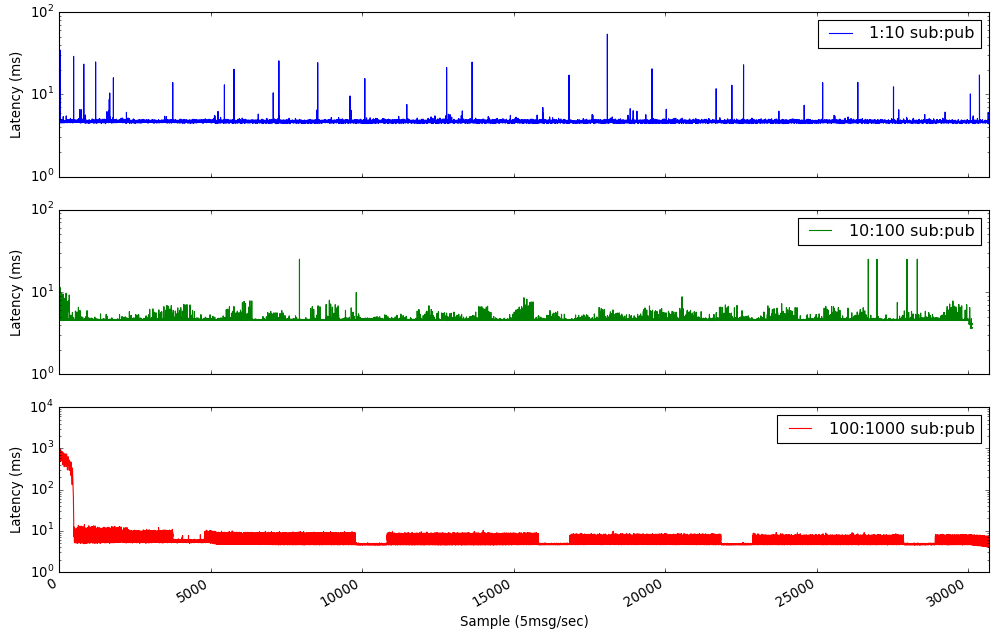
\includegraphics[width=\linewidth]{figs/singlenodelatency.png}
\caption{Microbenchmark: standalone CQBS broker forwarding latency with increasing concurrency}
\label{fig:singlenodelatency}
\end{figure}

First, we examine the latencies of the CQBS broker's forwarding mechanism in isolation -- without the communication overhead imposed by the fully replicated system.
We run a single broker on a \texttt{t2.medium} instance, backed by MongoDB.
Using a ratio of 10 publishers to one subscriber, we run three benchmarks with 1, 10 and 100 subscribers (with 10, 100 and 1,000 publishers accordingly).
Each publisher sends 5 messages per second; after the initial registration message (the high latencies at the beginning of each benchmark), each publisher sends only its stream UUID and an increasing counter as its value.
Each group of publishers/subscribers use entirely isolated sets of keys, so that they do not explicitly interfere with each other in the broker.
These three microbenchmarks are shown in Figure~\ref{fig:singlenodelatency}, and demonstrate that the latency is fairly consistent as the amount of concurrency scales.

The spikes in latency seen in the $N=1,10$ graphs are due to the pauses enacted by Go's garbage collection.
Fortunately, these do not affect the vast majority of requests.
For the $N=1,10$ cases, the mean latencies, 95\textsuperscript{th} percentile latencies and standard deviation are $4.67ms/4.85ms/0.55ms$ and $4.62ms/4.77ms/0.37ms$ respectively.
For the $N=100$ case, the garbage collection becomes more visible in the variability of response times, with mean, 95\textsuperscript{th} percentile and standard deviation latencies of $13.58ms/8.87ms/67.13ms$.
The troughs in the $N=100$ case are an odd phenomenon, most likely caused by garbage collection in the single Go process used to generate the 100 subscribers and 1000 publishers, generating approximately 5000 messages per second.

\subsection{Client Complexity}

\subsection{Fault Tolerance}
